\documentclass[11pt,a4paper]{article}

\usepackage{amsmath}
\usepackage{amssymb}
\usepackage{geometry}
\usepackage{tikz}
\usetikzlibrary{positioning}
\usepackage{siunitx}
\usepackage{booktabs}
\usepackage{hyperref}
\usepackage{microtype}
\usepackage{parskip}

\geometry{margin=2.5cm}

\sisetup{
  separate-uncertainty,
  per-mode=symbol
}

\hypersetup{
  colorlinks=true,
  linkcolor=black,
  urlcolor=blue
}

% --- tiny schematic helpers (plain TikZ) -------------------------------
\newcommand{\hres}[4]{% x, y, name, label   (horizontal resistor, 0.9 cm long)
  \node[draw,fill=white,minimum width=0.9cm,minimum height=0.3cm,inner sep=0] (#3) at (#1,#2) {};
  \node[font=\scriptsize,above=1pt of #3] {#4};}
\newcommand{\vres}[4]{% vertical resistor, 0.9 cm long
  \node[draw,fill=white,minimum width=0.3cm,minimum height=0.9cm,inner sep=0] (#3) at (#1,#2) {};
  \node[font=\scriptsize,right=2pt of #3] {#4};}
\newcommand{\hcap}[3]{% x, y, label   (series capacitor, plates vertical)
  \draw[thick] (#1-0.06,#2-0.3)--(#1-0.06,#2+0.3);
  \draw[thick] (#1+0.06,#2-0.3)--(#1+0.06,#2+0.3);
  \node[font=\scriptsize,above=4pt] at (#1,#2+0.3) {#3};}
\newcommand{\vcap}[4]{% shunt capacitor, plates horizontal
  \draw[thick] (#1-0.3,#2-0.06)--(#1+0.3,#2-0.06);
  \draw[thick] (#1-0.3,#2+0.06)--(#1+0.3,#2+0.06);
  \node[font=\scriptsize,right=6pt] at (#1+0.3,#2) {#4};}
\newcommand{\dotnode}[2]{\fill (#1,#2) circle (1.5pt);}

\title{Signal Processing of the Inclination Meter\\
       from DDS Excitation to Displacement Readout}
\author{}
\date{Draft --- work in progress}

\begin{document}

\maketitle
\tableofcontents
\bigskip

% ─────────────────────────────────────────────────────────────
\section{Scope and Conventions}
% ─────────────────────────────────────────────────────────────

This note describes the measurement signal chain of the REV~B instrument,
from the sine wave generated by the DDS to the displacement value delivered
by the firmware.  It aims to be unambiguous: every quantity has a name, a
unit, a sign convention and a place in the chain.  The chain is developed
one stage at a time.  This part covers the \emph{excitation}: the DDS up to
the two antiphase voltages~$A$ and~$B$ at the op-amp outputs, and how these
are attenuated, filtered and fed into the ADC.  It then introduces the Wyler
Leveltronic sensor, treated as a black box, and how its output is filtered
and fed into the ADC.  The remaining sections cover the sampling, the
amplitude and phase estimate, the complex ratio, and the processing that
follows it, and end with a list of open items and proposals.

\textbf{Sources.}  Component values come from the KiCad schematic
(\texttt{SignalProcessing.kicad\_sch}), \emph{except} where the built REV~B
boards differ from it; such deviations are stated explicitly (currently R52,
R46--R49).  Device figures come from the AD9833, AD826 and ADS131M04
datasheets.  Component
tolerances are not recorded in the schematic and are not used here.

\textbf{Conventions.}  All AC signals are sinusoids at the excitation
frequency~$f_0$.  Amplitudes are \emph{peak} values, not RMS.  Phases are
quoted relative to the DDS output; a positive phase means the signal leads.
Later parts re-reference phases to the ADC sampling grid.

% ─────────────────────────────────────────────────────────────
\section{Overview}
% ─────────────────────────────────────────────────────────────

\begin{center}
\small
\begin{tabular}{@{}lp{4.6cm}p{3.6cm}p{2.6cm}@{}}
\toprule
Stage & Parts & Function & Output \\
\midrule
DDS        & U14 (AD9833)     & 10-bit sine, $f_0 \approx \SI{2604}{\hertz}$ & --- \\
Filter     & C59, R50, R51, C60, C61 & DC block + RC low-pass ($R_{52}=0$) & \texttt{SineSignal} \\
Gain stage & U16A, R53, R54   & non-inverting, $G_1 = +11$ & \texttt{ExciterA} \\
Inverter   & U16B, R55, R56   & inverting, $G_2 = -1$      & \texttt{ExciterB} \\
A/B input network & R36, R38, R40, C53, R44, R48, C57 (A); R37, R39, R41, C54, R45, R49, C58 (B)
           & attenuator, AC coupling, RC filter & ADC pins AIN2P (A), AIN1P (B) \\
Sensor input network & C51, R42, D5--D8, R46, C55 (S1); C52, R43, D9--D12, R47, C56 (S2)
           & ground reference, clamps, RC filter & ADC pins AIN3P (S1), AIN0P (S2) \\
\bottomrule
\end{tabular}
\end{center}

The op-amp U16 (AD826, dual) runs from \SI{+5}{\volt} and \SI{-4.5}{\volt}
rails; the reference for all AC signals is ground.

% ─────────────────────────────────────────────────────────────
\section{Sine Generation (DDS)}
% ─────────────────────────────────────────────────────────────

The AD9833 is clocked by a timer output (TIM1 channel~4) at
$f_{\mathrm{MCLK}} = \SI{64}{\mega\hertz}/12 = \SI{5.3333}{\mega\hertz}$
and programmed once at boot with $\mathrm{FREQREG}=2^{17}$.  Exactly 2048
MCLK cycles make one period:
\begin{equation}
  \boxed{f_0 = f_{\mathrm{MCLK}}/2^{11} = \SI{2604.17}{\hertz}.}
  \label{eq:f0}
\end{equation}

The output pin is a $\SI{200}{\ohm}$ source delivering a \emph{unipolar}
sine.  From the datasheet limits ($\SI{38}{\milli\volt}$ to
$\SI{650}{\milli\volt}$) it has a DC offset of \SI{344}{\milli\volt} and a
peak amplitude
\begin{equation}
  V_d = \SI{306}{\milli\volt}.
\end{equation}
These are typical values with no guaranteed tolerance, and \texttt{VOUT}
drifts by about \SI{200}{ppm\per\celsius}.  The absolute amplitude is
therefore \emph{not} a calibrated quantity; the measurement is designed so
that it cancels (ratio stage, later part).

The DAC is 10~bit and updates at $f_{\mathrm{MCLK}}$, so the output is a
staircase with spectral images at $k f_{\mathrm{MCLK}}\pm f_0$.  Removing
them is one job of the filter.

% ─────────────────────────────────────────────────────────────
\section{Passive Filter}
% ─────────────────────────────────────────────────────────────

\begin{figure}[ht]
\centering
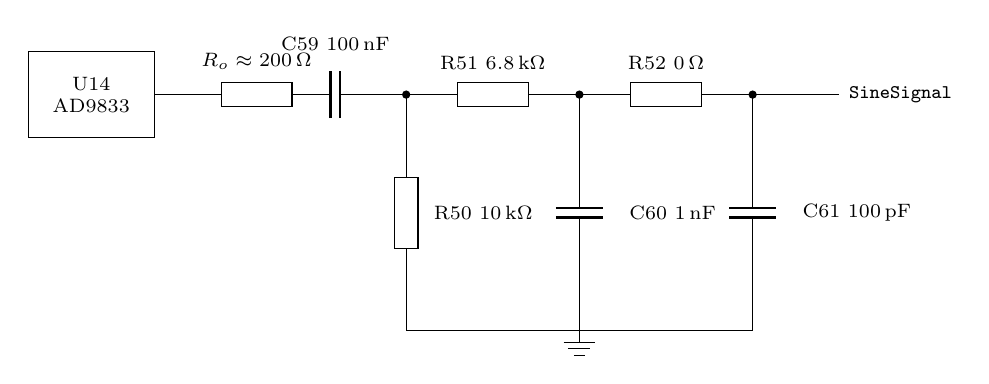
\begin{tikzpicture}[>=stealth]
  % DDS block and source resistance
  \node[draw,minimum width=1.6cm,minimum height=1.1cm,font=\scriptsize,align=center]
       (dds) at (-1.2,3.0) {U14\\AD9833};
  \hres{0.9}{3.0}{ro}{$R_o\approx\SI{200}{\ohm}$}
  \draw (dds.east) -- (ro.west);
  % signal rail y = 3
  \hcap{1.9}{3.0}{C59 \SI{100}{\nano\farad}}
  \draw (ro.east) -- (1.84,3.0);
  \draw (1.96,3.0) -- (2.8,3.0);
  \dotnode{2.8}{3.0}
  \draw (2.8,3.0) -- (3.45,3.0);
  \hres{3.9}{3.0}{r51}{R51 \SI{6.8}{\kilo\ohm}}
  \draw (4.35,3.0) -- (5.0,3.0);
  \dotnode{5.0}{3.0}
  \draw (5.0,3.0) -- (5.65,3.0);
  \hres{6.1}{3.0}{r52}{R52 \SI{0}{\ohm}}
  \draw (6.55,3.0) -- (7.2,3.0);
  \dotnode{7.2}{3.0}
  \draw (7.2,3.0) -- (8.3,3.0) node[right,font=\scriptsize] {\texttt{SineSignal}};
  % shunt elements
  \vres{2.8}{1.5}{r50}{R50 \SI{10}{\kilo\ohm}}
  \draw (2.8,3.0) -- (r50.north); \draw (r50.south) -- (2.8,0);
  \vcap{5.0}{1.5}{}{C60 \SI{1}{\nano\farad}}
  \draw (5.0,3.0) -- (5.0,1.56); \draw (5.0,1.44) -- (5.0,0);
  \vcap{7.2}{1.5}{}{C61 \SI{100}{\pico\farad}}
  \draw (7.2,3.0) -- (7.2,1.56); \draw (7.2,1.44) -- (7.2,0);
  % ground rail
  \draw (2.8,0) -- (7.2,0);
  \draw (5.0,0) -- (5.0,-0.15);
  \draw (4.8,-0.15) -- (5.2,-0.15); \draw (4.86,-0.23) -- (5.14,-0.23);
  \draw (4.93,-0.31) -- (5.07,-0.31);
\end{tikzpicture}
\caption{Filter between the DDS and the op-amp, as built on REV~B.  The
         schematic file still shows $R_{52}=\SI{68}{\kilo\ohm}$; on the
         boards it is bridged ($\SI{0}{\ohm}$), so C60 and C61 are in
         parallel.}
\label{fig:filter}
\end{figure}

\textbf{R52 is bridged on REV~B.}  The schematic shows R52 as
\SI{68}{\kilo\ohm}, which would make a two-stage RC filter.  On the built
boards it is $\SI{0}{\ohm}$, because the \SI{68}{\kilo\ohm} sat in the
op-amp's bias-current path and caused a large DC offset (section~\ref{sec:dc}).
This is a REV~B hardware workaround.  With it, C60 and C61 are in parallel,
$C_p = \SI{1.1}{\nano\farad}$, and the filter has two parts:
\begin{itemize}
  \item \textbf{DC block} (C59, R50): removes the DDS offset; high-pass
        corner about \SI{156}{\hertz}.
  \item \textbf{RC low-pass} (R51, $C_p$): a single first-order stage,
        $f_{\mathrm{LP}} = 1/(2\pi R_{51}C_p) = \SI{21.3}{\kilo\hertz}$.
\end{itemize}

Solving the network exactly (including the \SI{200}{\ohm} source and the
loading of R50, R51 and $C_p$; the op-amp input is treated as an open
circuit) gives, at $f_0$:

\begin{center}
\begin{tabular}{@{}lrr@{}}
\toprule
 & Magnitude & Phase \\
\midrule
DC block                 & 0.968 & $\SI{+3.3}{\degree}$ \\
Low-pass                 & 0.993 & $\SI{-7.0}{\degree}$ \\
\midrule
\textbf{Filter total}    & \textbf{0.961} & $\boldsymbol{\SI{-3.7}{\degree}}$ \\
\bottomrule
\end{tabular}
\end{center}

Above the corner the roll-off is first order.  At $f_{\mathrm{MCLK}}$ the
filter attenuates by only about \SI{48}{\decibel} (the original two-stage
design gave about \SI{95}{\decibel}), so the DAC images reach the op-amp
only mildly suppressed.  Whether this matters depends on the ADC's own
filtering and is treated in the acquisition part.

% ─────────────────────────────────────────────────────────────
\section{Gain Stage and Inverter}
% ─────────────────────────────────────────────────────────────

\begin{figure}[ht]
\centering
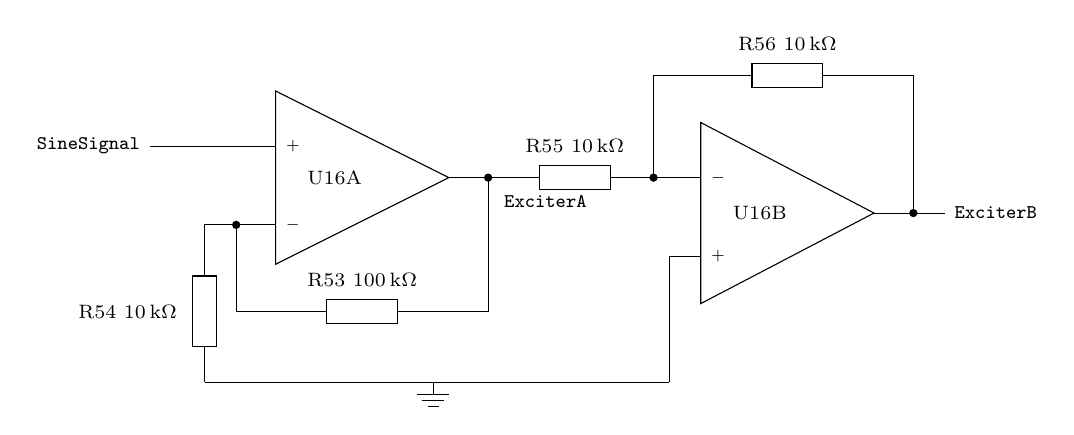
\begin{tikzpicture}[>=stealth]
  % ---- U16A, non-inverting ----
  \draw (-1.6,3.0) node[left,font=\scriptsize] {\texttt{SineSignal}} -- (0,3.0);
  \draw (0,3.7) -- (0,1.5) -- (2.2,2.6) -- cycle;
  \node[font=\tiny] at (0.22,3.0) {$+$};
  \node[font=\tiny] at (0.22,2.0) {$-$};
  \node[font=\scriptsize] at (0.75,2.6) {U16A};
  % inverting input node and R54 to ground
  \draw (0,2.0) -- (-0.5,2.0);
  \dotnode{-0.5}{2.0}
  \draw (-0.5,2.0) -- (-0.9,2.0) -- (-0.9,1.35);
  \vres{-0.9}{0.9}{r54}{}
  \node[font=\scriptsize,left=2pt of r54] {R54 \SI{10}{\kilo\ohm}};
  \draw (-0.9,0.45) -- (-0.9,0);
  % feedback R53
  \draw (2.2,2.6) -- (2.7,2.6);
  \dotnode{2.7}{2.6}
  \draw (2.7,2.6) -- (2.7,0.9) -- (1.55,0.9);
  \hres{1.1}{0.9}{r53}{R53 \SI{100}{\kilo\ohm}}
  \draw (0.65,0.9) -- (-0.5,0.9) -- (-0.5,2.0);
  % ---- R55 and U16B, inverting ----
  \draw (2.7,2.6) -- (3.35,2.6);
  \hres{3.8}{2.6}{r55}{R55 \SI{10}{\kilo\ohm}}
  \draw (4.25,2.6) -- (5.4,2.6);
  \dotnode{4.8}{2.6}
  \draw (5.4,3.3) -- (5.4,1.0) -- (7.6,2.15) -- cycle;
  \node[font=\tiny] at (5.62,2.6) {$-$};
  \node[font=\tiny] at (5.62,1.6) {$+$};
  \node[font=\scriptsize] at (6.15,2.15) {U16B};
  \draw (5.4,1.6) -- (5.0,1.6) -- (5.0,0);
  % feedback R56
  \draw (4.8,2.6) -- (4.8,3.9) -- (6.05,3.9);
  \hres{6.5}{3.9}{r56}{R56 \SI{10}{\kilo\ohm}}
  \draw (6.95,3.9) -- (8.1,3.9) -- (8.1,2.15);
  \draw (7.6,2.15) -- (8.5,2.15) node[right,font=\scriptsize] {\texttt{ExciterB}};
  \dotnode{8.1}{2.15}
  \node[font=\scriptsize,anchor=north west] at (2.78,2.5) {\texttt{ExciterA}};
  % ground rail
  \draw (-0.9,0) -- (5.0,0);
  \draw (2.0,0) -- (2.0,-0.15);
  \draw (1.8,-0.15) -- (2.2,-0.15); \draw (1.86,-0.23) -- (2.14,-0.23);
  \draw (1.93,-0.31) -- (2.07,-0.31);
\end{tikzpicture}
\caption{The two op-amp stages (U16A non-inverting, U16B inverting).
         Supplies: \texttt{5V0} on pin~8, \texttt{-4V5} on pin~4.}
\label{fig:opamp}
\end{figure}

\textbf{U16A (non-inverting).}  The filtered sine enters the non-inverting
input; R53 and R54 set
\begin{equation}
  G_1 = 1 + R_{53}/R_{54} = 11 .
\end{equation}
The output is the net \texttt{ExciterA}.  The AD826 (\SI{50}{\mega\hertz}
gain-bandwidth product) is far faster than needed: at $f_0$ its phase error
is about \SI{0.03}{\degree}, which is ignored.

\textbf{U16B (inverting).}  R55 and R56 (both \SI{10}{\kilo\ohm}) make a
unity-gain inverter, $G_2 = -R_{56}/R_{55} = -1$, whose output is
\texttt{ExciterB}.  So $B$ has the same amplitude as $A$ and is exactly
\SI{180}{\degree} out of phase, up to the ratio $R_{56}/R_{55}$.  Any common
change (DDS amplitude, filter, $G_1$) scales $A$ and $B$ identically; only
the resistor ratio makes them differ.  The ratio calculation in the digital
part relies on this.

\textbf{Result.}
\begin{equation}
  \boxed{\;|V_A| = |V_B| = G_1\cdot 0.961\cdot V_d
    = 11\cdot 0.961\cdot\SI{0.306}{\volt} \approx \SI{3.23}{\volt}\ \text{(peak)},\;}
\end{equation}
with phases $\varphi_A=\SI{-3.7}{\degree}$ and
$\varphi_B=\SI{+176.3}{\degree}$ relative to the DDS output.

% ─────────────────────────────────────────────────────────────
\section{DC Operating Point}
\label{sec:dc}
% ─────────────────────────────────────────────────────────────

The AD826 has bipolar inputs drawing a bias current of
\SI{3.3}{\micro\ampere} (typical, \SI{6.6}{\micro\ampere} maximum).  The
capacitors block DC, so this current must flow to ground through R50, R51
and R52.  The voltage it develops across that resistance is amplified by
$G_1$ and appears as a DC offset on \texttt{ExciterA} (and, inverted, on
\texttt{ExciterB}):

\begin{center}
\begin{tabular}{@{}lrrr@{}}
\toprule
 & DC path resistance & Offset, \SI{3.3}{\micro\ampere} & Offset, \SI{6.6}{\micro\ampere} \\
\midrule
Schematic, $R_{52}=\SI{68}{\kilo\ohm}$ & \SI{84.8}{\kilo\ohm} & \SI{-2.75}{\volt} & \SI{-5.5}{\volt} \\
REV B, $R_{52}=\SI{0}{\ohm}$           & \SI{16.8}{\kilo\ohm} & \SI{-0.28}{\volt} & \SI{-0.56}{\volt} \\
\bottomrule
\end{tabular}
\end{center}

With the schematic value, the \SI{3.23}{\volt} AC peak on a
\SI{-2.75}{\volt} offset would need about \SI{-6}{\volt}, beyond the
\SI{-4.5}{\volt} rail; this was seen as a DC offset problem on the board and
is why R52 was bridged.

With $R_{52}=0$ the residual offset is small, but headroom on the negative
peak of \texttt{ExciterA} (positive peak of \texttt{ExciterB}) is still
thin: about \SI{3.5}{\volt} are needed, against an AD826 output swing of
$\pm\SI{3.3}{\volt}$ (guaranteed) to $\pm\SI{3.8}{\volt}$ (typical).
\textbf{Status:} reported to work; DC level and peak values on the two nets
have not been measured yet and should be recorded here once they are.

% ─────────────────────────────────────────────────────────────
\section{Attenuator and ADC Input Filter (Channels A and B)}
% ─────────────────────────────────────────────────────────────

\begin{figure}[ht]
\centering
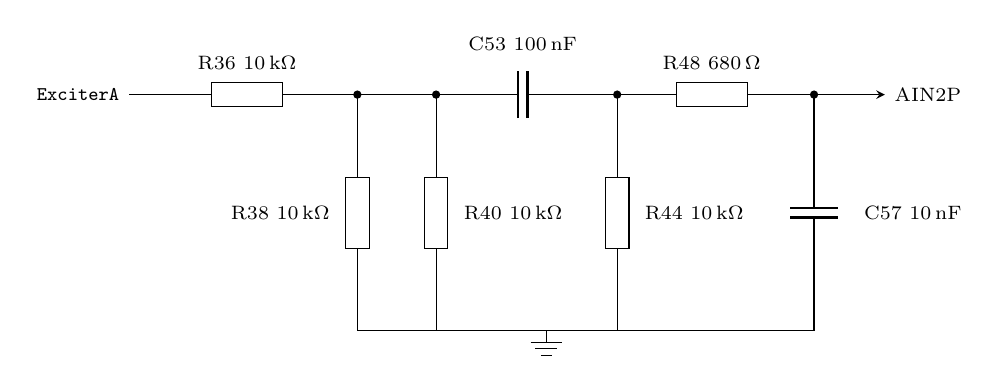
\begin{tikzpicture}[>=stealth]
  \draw (-0.3,3.0) node[left,font=\scriptsize] {\texttt{ExciterA}} -- (0.75,3.0);
  \hres{1.2}{3.0}{r36}{R36 \SI{10}{\kilo\ohm}}
  \draw (1.65,3.0) -- (4.64,3.0);
  \dotnode{2.6}{3.0}\dotnode{3.6}{3.0}
  % divider shunts R38, R40
  \vres{2.6}{1.5}{r38}{}
  \node[font=\scriptsize,left=2pt of r38] {R38 \SI{10}{\kilo\ohm}};
  \vres{3.6}{1.5}{r40}{R40 \SI{10}{\kilo\ohm}}
  \draw (2.6,3.0) -- (r38.north); \draw (r38.south) -- (2.6,0);
  \draw (3.6,3.0) -- (r40.north); \draw (r40.south) -- (3.6,0);
  % C53
  \hcap{4.7}{3.0}{C53 \SI{100}{\nano\farad}}
  \draw (4.76,3.0) -- (7.55,3.0);
  \dotnode{5.9}{3.0}
  \vres{5.9}{1.5}{r44}{R44 \SI{10}{\kilo\ohm}}
  \draw (5.9,3.0) -- (r44.north); \draw (r44.south) -- (5.9,0);
  % R48
  \hres{7.1}{3.0}{r48}{R48 \SI{680}{\ohm}}
  \draw (r48.east) -- (8.4,3.0);
  \dotnode{8.4}{3.0}
  \vcap{8.4}{1.5}{}{C57 \SI{10}{\nano\farad}}
  \draw (8.4,3.0) -- (8.4,1.56); \draw (8.4,1.44) -- (8.4,0);
  \draw[->] (8.4,3.0) -- (9.3,3.0) node[right,font=\scriptsize] {AIN2P};
  % ground rail
  \draw (2.6,0) -- (8.4,0);
  \draw (5.0,0) -- (5.0,-0.15);
  \draw (4.8,-0.15) -- (5.2,-0.15); \draw (4.86,-0.23) -- (5.14,-0.23);
  \draw (4.93,-0.31) -- (5.07,-0.31);
\end{tikzpicture}
\caption{Input network of channel~A, as built on REV~B (R48 is
         \SI{680}{\ohm}, not the \SI{680}{\kilo\ohm} of the schematic).
         Channel~B is identical (R37, R39, R41, C54, R45, R49, C58) and
         ends at AIN1P.  The ADC's negative inputs are tied to ground.}
\label{fig:abinput}
\end{figure}

\textbf{REV~B deviation.}  The schematic and the manufactured boards
specify R48 and R49 as \SI{680}{\kilo\ohm}.  This was a mistake: with
\SI{10}{\nano\farad} it gives a corner of \SI{23}{\hertz} and would leave
almost none of the \SI{2.6}{\kilo\hertz} signal at the ADC.  The working
boards carry \SI{680}{\ohm} instead (hardware rework), which is what is
described here.

\textbf{What the parts do.}
\begin{itemize}
  \item \textbf{R36 with R38$\parallel$R40} (\SI{10}{\kilo\ohm} over
        \SI{5}{\kilo\ohm}): attenuator, ratio $1/3$.  It brings the
        \SI{3.2}{\volt} peak of the exciter into the ADC's $\pm\SI{1.2}{\volt}$
        range.  The firmware constant for this attenuator is 3.000
        (\texttt{disp\_atten\_milli}).
  \item \textbf{C53 with R44:} AC coupling.  C53 removes the DC offset of
        the exciter (section~\ref{sec:dc}); R44 gives the node a DC path to
        ground.  R44 also loads the attenuator, so the total division is
        larger than $1/3$.
  \item \textbf{R48 with C57:} RC low-pass directly at the ADC pin, with an
        isolated corner of $1/(2\pi\cdot\SI{680}{\ohm}\cdot\SI{10}{\nano\farad})
        = \SI{23.4}{\kilo\hertz}$.
\end{itemize}

\textbf{The stages are not independent.}  Since R48 is small, C57 is not
isolated from R44: the node after C53 sees R44 in parallel with R48+C57.  The
effective low-pass corner is therefore set mostly by the source resistance
in front of C57 ($R_{36}\parallel R_{38}\parallel R_{40}\parallel R_{44}
\approx\SI{2.5}{\kilo\ohm}$, plus R48), giving about \SI{5}{\kilo\hertz},
not \SI{23}{\kilo\hertz}.  Solving the network exactly (ADC input treated as
an open circuit) gives a band-pass response with its maximum
(gain 0.231) near \SI{0.8}{\kilo\hertz} and its $\SI{-3}{\decibel}$ points at
\SI{108}{\hertz} and \SI{5.5}{\kilo\hertz}.  At the excitation frequency,
on the upper skirt of that band:
\begin{equation}
  \boxed{H_{AB}(\mathrm{j}\omega_0) = 0.212\;\angle\,\SI{-23.7}{\degree}
  \quad(\SI{-13.5}{\decibel}).}
\end{equation}
At $f_{\mathrm{MCLK}}$ the network attenuates by a further
\SI{73}{\decibel} (on top of the \SI{48}{\decibel} of the first filter).
Channels A and B use identical networks, so this gain and phase are common
to both.  They matter as soon as A or B is compared with a differently
filtered channel, such as the sensor inputs.

\textbf{ADC input.}  Each channel is single-ended: the positive input sees
the network output, the negative input is grounded.  The PGA gain of the A
and B channels is~1, so the full-scale range is $\pm\SI{1.2}{\volt}$ and one
code (LSB) is $2.4\,\mathrm{V}/2^{24}=\SI{143}{\nano\volt}$.  The ADC's
input impedance at gain~1 is \SI{330}{\kilo\ohm} at a modulator frequency of
\SI{4.096}{\mega\hertz} and scales inversely with it, so about
\SI{510}{\kilo\ohm} here (Section~10).  This is large against R48; including
it changes the result by less than 1\,\% and it is ignored.  The expected
amplitude at the ADC pin is
\begin{equation}
  |V_{A,\mathrm{pin}}| = |V_{B,\mathrm{pin}}| = 0.212\cdot\SI{3.23}{\volt}
  \approx \SI{0.68}{\volt}\ \text{(peak)},
\end{equation}
about 57\,\% of full scale, leaving a factor of $1.75$ headroom.

\textbf{Cross-check with the firmware.}  The firmware reports about
\SI{885}{\milli\volt} RMS for channel~A, i.e.\ \SI{1.25}{\volt} peak.  That
would exceed the $\pm\SI{1.2}{\volt}$ range, and yet no clipping is
counted.  The reason is a unit factor: the firmware diagnostic
(\texttt{phasor\_peak\_mv} in \texttt{svc\_displacement.c}) converts codes
with $2400/\mathrm{PGA}/2^{23}$, twice the datasheet LSB.  With the
datasheet LSB the measured peak is about \SI{0.63}{\volt}, \SI{9}{\percent}
below the prediction above --- consistent within the unspecified DDS
amplitude tolerance (the prediction uses the typical DDS amplitude).
\textbf{Open:} the firmware scaling should be confirmed and, if wrong,
corrected; the values in this note use the datasheet LSB.

% ─────────────────────────────────────────────────────────────
\section{The Sensor: Wyler Leveltronic A40 (Black Box)}
% ─────────────────────────────────────────────────────────────

The sensor is a Wyler Leveltronic A40 inclination sensor in its
\SI{5}{\micro\metre\per\metre}-per-digit version (source: the Wyler
operating manual, 06/87).  It is treated here as a black box; only its
electrical behaviour at the terminals matters.

\textbf{Principle, in brief.}  A mass disc of about \SI{1}{\gram} hangs on leaf
springs between two electrodes, forming a differential capacitor; air
damping and the friction-free suspension give the good repeatability.
Tilting the instrument moves the disc toward one electrode and away from the
other.  The original electronics (Levelmeter~25) is a carrier-frequency
system ($\SI{2.5}{\kilo\hertz}$) with phase-sensitive rectification.  In this
instrument that job is done by the ADC and the digital processing instead.

\begin{figure}[ht]
\centering
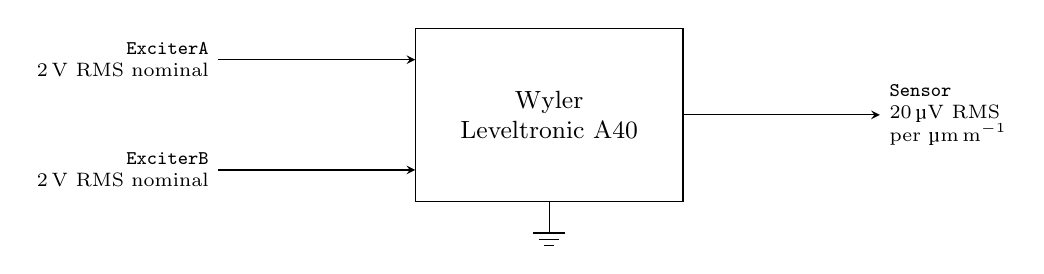
\begin{tikzpicture}[>=stealth]
  \node[draw,minimum width=3.4cm,minimum height=2.2cm,align=center,font=\small]
       (box) at (0,0) {Wyler\\Leveltronic A40};
  \draw[->] (-4.2,0.7) node[left,font=\scriptsize,align=right] {\texttt{ExciterA}\\$\SI{2}{\volt}$ RMS nominal} -- (-1.7,0.7);
  \draw[->] (-4.2,-0.7) node[left,font=\scriptsize,align=right] {\texttt{ExciterB}\\$\SI{2}{\volt}$ RMS nominal} -- (-1.7,-0.7);
  \draw[->] (1.7,0) -- (4.2,0) node[right,font=\scriptsize,align=left] {\texttt{Sensor}\\$\SI{20}{\micro\volt}$ RMS\\per $\si{\micro\metre\per\metre}$};
  \draw (0,-1.1) -- (0,-1.5);
  \draw (-0.2,-1.5) -- (0.2,-1.5); \draw (-0.13,-1.58) -- (0.13,-1.58);
  \draw (-0.06,-1.66) -- (0.06,-1.66);
\end{tikzpicture}
\caption{The sensor as a black box: two antiphase supply inputs and one
         signal output, plus ground.}
\label{fig:sensor}
\end{figure}

\subsection{Electrical behaviour}

\begin{itemize}
  \item \textbf{Powered by the exciter signals.}  The sensor has no other
        supply.  It is fed directly with the two antiphase excitation
        voltages $A$ and $B$ (\SI{2}{\volt} RMS at \SI{2.5}{\kilo\hertz}
        nominal in the manual).  Their generation is described in the
        sections above.
  \item \textbf{The output is a sine wave} at the excitation frequency.  Its
        amplitude is proportional to the magnitude of the tilt.
  \item \textbf{The sign of the tilt is the phase of the output relative to
        $A$ and $B$.}  For one sign the output is in phase with $A$ (and so
        in antiphase with $B$); for the other sign it is in phase with $B$.
        The output passes through zero amplitude at zero tilt.
  \item \textbf{Sensitivity:} \SI{20}{\micro\volt} RMS per
        \SI{0.001}{\milli\metre\per\metre} (that is, per
        $\SI{1}{\micro\metre\per\metre}$) for the
        \SI{5}{\micro\metre\per\metre}-per-digit version, which is the one
        used here.  This agrees with the manual's \SI{100}{\micro\volt} RMS
        per digit of $\SI{5}{\micro\metre\per\metre}$.
\end{itemize}

\subsection{Model}

Let $\tau$ be the tilt in $\si{\micro\metre\per\metre}$, positive when the
output is in phase with~$A$, and let $\underline{V}_S$ be the phasor of the
sensor output.  Since $\underline{V}_B=-\underline{V}_A$, the behaviour above
is described by a single real number per unit tilt:
\begin{equation}
  \underline{V}_S = \kappa\,\tau\,\underline{V}_A,
  \qquad \kappa \approx \frac{\SI{20}{\micro\volt}}{\SI{2}{\volt}}
  = 10^{-5}\ \text{per}\ \si{\micro\metre\per\metre}.
  \label{eq:sensor}
\end{equation}
A positive $\tau$ gives $\underline{V}_S$ in phase with $\underline{V}_A$, a
negative $\tau$ in phase with $\underline{V}_B$.  Equation~\eqref{eq:sensor}
also shows that the output is \emph{ratiometric}: it scales with the
excitation amplitude, so the ratio $\underline{V}_S/\underline{V}_A$ measures
the tilt independent of that amplitude.  (This is an inference from the
sensor being supplied by the exciter, with the nominal figures taken at
\SI{2}{\volt}.)

Three points on how this maps to the present instrument:
\begin{itemize}
  \item The excitation here is $\SI{2.29}{\volt}$ RMS at
        $\SI{2.604}{\kilo\hertz}$, i.e.\ 14\,\% above the nominal supply
        and 4\,\% above the nominal carrier frequency.  With
        \eqref{eq:sensor} the expected sensitivity is about
        $\SI{23}{\micro\volt}$ RMS per $\si{\micro\metre\per\metre}$ at
        the sensor output, to be verified.
  \item The sign convention $\tau>0 \Leftrightarrow$ output in phase with
        $A$ is the \emph{electrical} one.  Which physical direction is
        positive depends on how the instrument is mounted and is fixed per
        instrument during calibration.
  \item The manual specifies a range of $\pm1999$ digits, i.e.\
        $\pm\SI{10}{\milli\metre\per\metre}$ for this version, which
        corresponds to about $\SI{200}{\milli\volt}$ RMS at the sensor
        output (at nominal excitation).
\end{itemize}

How the sensor output reaches the ADC is described in the next section.

% ─────────────────────────────────────────────────────────────
\section{Sensor Input Network and ADC (Channels S1 and S2)}
% ─────────────────────────────────────────────────────────────

Two sensors can be connected.  The output of sensor~1 (net \texttt{Sensor1},
connector J5) goes through the network of Figure~\ref{fig:sinput} to ADC
input AIN3P (channel~3); sensor~2 (\texttt{Sensor2}, J6) has an identical
network (C52, R43, D9--D12, R47, C56) into AIN0P (channel~0).  As for A and B,
the ADC's negative inputs are grounded.

\begin{figure}[ht]
\centering
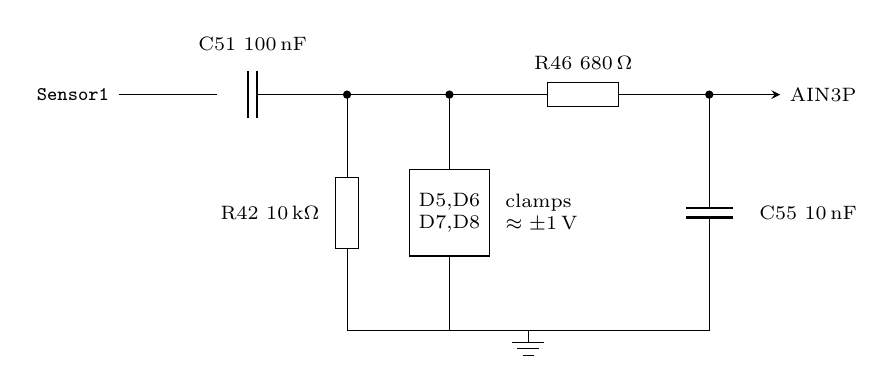
\begin{tikzpicture}[>=stealth]
  \draw (-0.3,3.0) node[left,font=\scriptsize] {\texttt{Sensor1}} -- (0.95,3.0);
  \hcap{1.4}{3.0}{C51 \SI{100}{\nano\farad}}
  \draw (1.46,3.0) -- (5.15,3.0);
  \dotnode{2.6}{3.0}\dotnode{3.9}{3.0}
  % R42 ground reference
  \vres{2.6}{1.5}{r42}{}
  \node[font=\scriptsize,left=2pt of r42] {R42 \SI{10}{\kilo\ohm}};
  \draw (2.6,3.0) -- (r42.north); \draw (r42.south) -- (2.6,0);
  % clamp block
  \node[draw,minimum width=0.9cm,minimum height=1.1cm,font=\scriptsize,align=center,fill=white] (clamp) at (3.9,1.5) {D5,D6\\D7,D8};
  \draw (3.9,3.0) -- (clamp.north); \draw (clamp.south) -- (3.9,0);
  \node[font=\scriptsize,right=2pt of clamp,align=left] {clamps\\$\approx\pm\SI{1}{\volt}$};
  % R46
  \hres{5.6}{3.0}{r46}{R46 \SI{680}{\ohm}}
  \draw (r46.east) -- (7.2,3.0);
  \dotnode{7.2}{3.0}
  \vcap{7.2}{1.5}{}{C55 \SI{10}{\nano\farad}}
  \draw (7.2,3.0) -- (7.2,1.56); \draw (7.2,1.44) -- (7.2,0);
  \draw[->] (7.2,3.0) -- (8.1,3.0) node[right,font=\scriptsize] {AIN3P};
  % ground rail
  \draw (2.6,0) -- (7.2,0);
  \draw (4.9,0) -- (4.9,-0.15);
  \draw (4.7,-0.15) -- (5.1,-0.15); \draw (4.76,-0.23) -- (5.04,-0.23);
  \draw (4.83,-0.31) -- (4.97,-0.31);
\end{tikzpicture}
\caption{Input network of sensor~1, as built on REV~B (R46 is
         \SI{680}{\ohm}, not the \SI{680}{\kilo\ohm} of the schematic).  Each
         clamp block is two series diodes (1N4148WS) each way: D5, D6 to
         ground for negative excursions, D8, D7 for positive ones.}
\label{fig:sinput}
\end{figure}

\textbf{REV~B deviation.}  As for R48 and R49, the schematic and the
manufactured boards specify R46 and R47 as \SI{680}{\kilo\ohm}, which was a
mistake (a \SI{23}{\hertz} corner with \SI{10}{\nano\farad}).  The working
boards carry \SI{680}{\ohm}.

\textbf{What the parts do.}
\begin{itemize}
  \item \textbf{C51 with R42: ground reference.}  The sensor signal is AC;
        C51 blocks any DC and R42 ties the node to ground, so the signal is
        centred on \SI{0}{\volt} at the ADC.  Together they form a high-pass
        with corner $1/(2\pi\cdot\SI{100}{\nano\farad}\cdot\SI{10}{\kilo\ohm})
        = \SI{159}{\hertz}$.
  \item \textbf{D5--D8: protection clamps.}  Two diode drops in each
        direction limit the node to roughly $\pm\SI{1}{\volt}$, below the
        ADC's absolute input limit.  In normal operation the signal is a few
        tens of millivolts and the diodes do not conduct.
  \item \textbf{R46 with C55: RC low-pass} at the ADC pin, isolated corner
        $1/(2\pi\cdot\SI{680}{\ohm}\cdot\SI{10}{\nano\farad})
        = \SI{23.4}{\kilo\hertz}$.
\end{itemize}

\textbf{Transfer function.}  Solving the network exactly, with the sensor
treated as an ideal low-impedance source and the ADC input as an open
circuit (its input impedance is at least \SI{1}{\mega\ohm} at gain~16), gives
a band-pass with maximum gain $0.904$ near \SI{1.9}{\kilo\hertz} and
$\SI{-3}{\decibel}$ points at \SI{143}{\hertz} and \SI{26}{\kilo\hertz}.  At
the excitation frequency
\begin{equation}
  \boxed{H_S(\mathrm{j}\omega_0) = 0.903\;\angle\,\SI{-2.6}{\degree}.}
\end{equation}
The response at $f_{\mathrm{MCLK}}$ is $\SI{-47}{\decibel}$.  This network is
much wider and much less attenuating than that of A and B
(Section~7), because no attenuator sits in front of it.  Two consequences:
\begin{itemize}
  \item \textbf{Gain:} $|H_S|=0.903$ holds only if the sensor output
        impedance is small.  A series source resistance of \SI{1}{\kilo\ohm}
        already lowers it to $0.81$.  The sensor's output impedance is not
        specified in the manual.
  \item \textbf{Phase:} the S network lags by $\SI{2.6}{\degree}$, the A/B
        network by $\SI{23.7}{\degree}$.  In the ADC domain the sensor
        signal therefore carries a phase offset of
        $\SI{+21}{\degree}$ relative to A and B, on top of anything the
        sensor itself adds.  The ratio calculation compares complex
        phasors, so this offset has to be accounted for in the digital
        processing.
\end{itemize}

\textbf{ADC input.}  Channels~3 and~0 run with a PGA gain of~16 (A and B: 1).
The full-scale range is therefore $\pm\SI{75}{\milli\volt}$ and one LSB is
$2.4\,\mathrm{V}/(16\cdot 2^{24}) = \SI{8.9}{\nano\volt}$.  With the
expected \SI{23}{\micro\volt} RMS per $\si{\micro\metre\per\metre}$ at the
sensor output (Section~8) and $|H_S|$, the sensitivity at the ADC pin is
\begin{equation}
  \approx \SI{21}{\micro\volt}\ \text{RMS per}\ \si{\micro\metre\per\metre},
\end{equation}
so full scale corresponds to about $\pm\SI{2.5}{\milli\metre\per\metre}$
tilt.  This is a quarter of the sensor's own $\pm\SI{10}{\milli\metre\per\metre}$
range; larger tilts need a lower PGA gain or would clip.

\textbf{Observed phase.}  The long granite-plate run (both sensors with a
large signal) shows the following average phase differences in the ADC
domain.  They are given as the \emph{delay} of the first signal behind the
second (positive = later); this is the angle the firmware's demodulator
reports (Section~11).

\begin{center}
\begin{tabular}{@{}lr@{}}
\toprule
Quantity & Measured \\
\midrule
$B$ behind $A$                   & $\SI{178.9}{\degree}$ (ideal: $\SI{180}{\degree}$) \\
$S_1$ behind $B$                 & $\SI{-10.0}{\degree}$ \\
$S_2$ behind $B$                 & $\SI{-13.8}{\degree}$ \\
\bottomrule
\end{tabular}
\end{center}

Both sensor signals were in phase with $B$ (negative tilt) to within about
$\SI{10}{\degree}$--$\SI{14}{\degree}$.  The networks alone delay the S
signal by $\SI{2.6}{\degree}$ and the A/B signals by $\SI{23.7}{\degree}$,
so the S signals should arrive $\SI{21}{\degree}$ \emph{earlier} than $B$
($-\SI{21}{\degree}$).  Measured are $-\SI{10}{\degree}$ and
$-\SI{14}{\degree}$, so about $\SI{+11}{\degree}$ ($S_1$) and
$\SI{+7}{\degree}$ ($S_2$) of additional delay remain that must come from
the sensor itself (its own phase lag or output impedance).
\textbf{Open:} this needs to be characterised; also the
$\SI{1}{\degree}$ deviation of $B$ from exactly $\SI{180}{\degree}$ relative
to $A$ is unexplained (candidates: resistor ratio, channel-to-channel timing
in the ADC).

\subsection{Phase calibration (planned)}

\textbf{Status: planned, not implemented.}  Nothing in the current firmware
needs to change for this note; it records the intended approach.

In theory $A$ and $B$ are exactly $\SI{180}{\degree}$ apart, and $S_1$ and
$S_2$ are either in phase with $A$ ($\SI{0}{\degree}$) or in phase with $B$
($\SI{180}{\degree}$), depending on the direction of tilt.  In the ADC domain
this is distorted by the input filters (different for the A/B and the S
paths), by the sensor itself and by further effects such as channel
timing.  The measured values above show the size of the distortion.

The intended remedy is an \emph{empirical} calibration of all four phases:
\begin{itemize}
  \item \textbf{Convention:} after calibration, $A$ reads
        $\SI{0}{\degree}$ and $B$ reads $\SI{180}{\degree}$.  Each sensor
        signal then lies on the real axis: $\SI{0}{\degree}$ for positive
        tilt (in phase with $A$), $\SI{180}{\degree}$ for negative tilt.
  \item \textbf{Four constants:} one phase correction per channel
        ($A$, $B$, $S_1$, $S_2$), determined by measurement and stored in
        EEPROM as calibration constants.  Each measured phasor is rotated by
        its constant before further processing.
  \item \textbf{Determination:} $A$ and $B$ are measured directly (this fixes
        the reference and the exact $B$--$A$ offset).  For $S_1$ and $S_2$ a
        clearly non-zero tilt is applied in a known direction, and the
        constant is chosen so that the signal lands on the real axis with the
        sign given by that direction.
\end{itemize}
Because the correction is applied after demodulation, it is independent of
where in the analog chain each phase shift arises.  The constants are valid
as long as the filters and the sensor do not change; they need to be
re-determined after any rework of the input networks, or if the phases turn
out to drift with temperature.  (Whether the absolute phase of $A$ is itself
reproducible from run to run is discussed in Section~10.5.)

% ─────────────────────────────────────────────────────────────
\section{Sampling}
% ─────────────────────────────────────────────────────────────

All four signals ($S_2$, $B$, $A$, $S_1$) are digitised by one
ADS131M04, a four-channel, 24-bit delta-sigma ADC with simultaneous
sampling.

\subsection{Clocks and locking to the sine}

The sampling rate is locked to the sine because both are derived from the
\emph{same} clock, with fixed integer ratios (Figure~\ref{fig:clocks}).  The
microcontroller's \SI{64}{\mega\hertz} system clock (from the
\SI{8}{\mega\hertz} crystal via the PLL) feeds two timers.  Each divides by 12
and outputs a \SI{5.3333}{\mega\hertz} square wave: TIM1 clocks the DDS
(Section~3), TIM2 clocks the ADC.

\begin{figure}[ht]
\centering
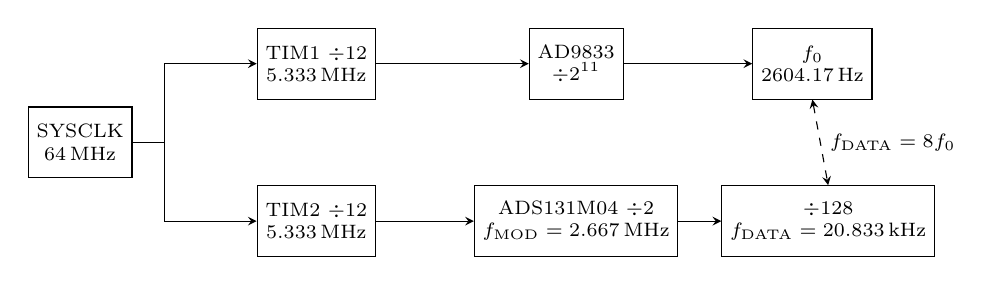
\begin{tikzpicture}[>=stealth,
    blk/.style={draw,minimum height=0.9cm,font=\scriptsize,align=center,inner sep=3pt}]
  \node[blk] (sys) at (0,0) {SYSCLK\\\SI{64}{\mega\hertz}};
  \node[blk] (t1) at (3.0,1.0) {TIM1 $\div 12$\\\SI{5.333}{\mega\hertz}};
  \node[blk] (dds) at (6.3,1.0) {AD9833\\$\div 2^{11}$};
  \node[blk] (f0) at (9.3,1.0) {$f_0$\\\SI{2604.17}{\hertz}};
  \node[blk] (t2) at (3.0,-1.0) {TIM2 $\div 12$\\\SI{5.333}{\mega\hertz}};
  \node[blk] (mod) at (6.3,-1.0) {ADS131M04 $\div 2$\\$f_{\mathrm{MOD}}=\SI{2.667}{\mega\hertz}$};
  \node[blk] (fd) at (9.5,-1.0) {$\div 128$\\$f_{\mathrm{DATA}}=\SI{20.833}{\kilo\hertz}$};
  \draw[->] (sys.east) -- ++(0.4,0) |- (t1.west);
  \draw[->] (sys.east) -- ++(0.4,0) |- (t2.west);
  \draw[->] (t1) -- (dds); \draw[->] (dds) -- (f0);
  \draw[->] (t2) -- (mod); \draw[->] (mod) -- (fd);
  \draw[<->,dashed] (f0.south) -- node[right,font=\scriptsize] {$f_{\mathrm{DATA}} = 8 f_0$} (fd.north);
\end{tikzpicture}
\caption{Clock tree.  DDS output and ADC sample rate come from the same
         \SI{64}{\mega\hertz} clock through fixed dividers.}
\label{fig:clocks}
\end{figure}

The DDS output frequency is $f_0=f_{\mathrm{MCLK}}/2^{11}$ (FREQREG $=2^{17}$).
The ADC runs its modulators at $f_{\mathrm{MOD}}=f_{\mathrm{CLKIN}}/2$, and the
firmware selects an oversampling ratio of $\mathrm{OSR}=128$ (register
\texttt{CLOCK}), so one conversion per channel is delivered at
\begin{equation}
  f_{\mathrm{DATA}} = \frac{f_{\mathrm{CLKIN}}}{2\,\mathrm{OSR}}
  = \frac{f_{\mathrm{CLKIN}}}{256} = \SI{20.833}{\kilo\hertz}
  = 8\,f_0 .
\end{equation}
Exactly \textbf{eight samples per sine period}, always: a change of the
crystal frequency (initial tolerance or temperature drift) moves $f_0$ and
$f_{\mathrm{DATA}}$ together.  There is no other oscillator and no software
timing involved in choosing the sampling instants.

The software only \emph{reads} conversions.  A third timer (TIM7) polls the
ADC's data-ready line at $2f_{\mathrm{DATA}}$ (also derived from the same
clock) and starts a DMA read of the 18-byte SPI frame
($\text{status}+4\times\text{24-bit data}+\text{CRC}$, about \SI{10}{\micro\second}
at \SI{16}{\mega\hertz}).  The data-ready line stays active until read, so a
late read delays a sample but never changes when it was taken.

\textbf{What is not locked.}  The \emph{phase} between the DDS sine and the
sample grid is fixed while the instrument runs, but arbitrary: it depends on
when each device was started.  Only phases of the four channels
\emph{relative to each other} are therefore meaningful in general (see
Section~10.5).

\subsection{Simultaneous sampling of the four channels}

The ADS131M04 contains four independent delta-sigma modulators with their
own digital filters, all running from the same modulator clock.  There is no
multiplexer: the four channels are converted in parallel and their results
are updated together, at the same falling edge of the data-ready line.  One
SPI frame therefore contains four samples that belong to the same instant.

\begin{center}
\begin{tabular}{@{}llll@{}}
\toprule
ADC channel & Pin & Signal & PGA gain \\
\midrule
CH0 & AIN0P & $S_2$ (sensor 2) & 16 \\
CH1 & AIN1P & $B$ & 1 \\
CH2 & AIN2P & $A$ & 1 \\
CH3 & AIN3P & $S_1$ (sensor 1) & 16 \\
\bottomrule
\end{tabular}
\end{center}
All negative inputs are grounded (single-ended use).  The chip also has
per-channel phase-delay registers; they are left at their default of zero,
so no artificial inter-channel delay exists.

\subsection{PGA gain and resolution}

Each channel has its own programmable-gain amplifier.  The available gains
and the resulting full-scale range (FSR $=\pm1.2\,\mathrm{V}/G$) and code size
(1\,LSB $=2.4\,\mathrm{V}/(G\cdot 2^{24})$) are:

\begin{center}
\small
\begin{tabular}{@{}rrr@{}}
\toprule
Gain $G$ & FSR (peak) & 1 LSB \\
\midrule
1   & $\pm\SI{1200}{\milli\volt}$  & \SI{143}{\nano\volt} \\
2   & $\pm\SI{600}{\milli\volt}$   & \SI{71.5}{\nano\volt} \\
4   & $\pm\SI{300}{\milli\volt}$   & \SI{35.8}{\nano\volt} \\
8   & $\pm\SI{150}{\milli\volt}$   & \SI{17.9}{\nano\volt} \\
16  & $\pm\SI{75}{\milli\volt}$    & \SI{8.94}{\nano\volt} \\
32  & $\pm\SI{37.5}{\milli\volt}$  & \SI{4.47}{\nano\volt} \\
64  & $\pm\SI{18.75}{\milli\volt}$ & \SI{2.24}{\nano\volt} \\
128 & $\pm\SI{9.375}{\milli\volt}$ & \SI{1.12}{\nano\volt} \\
\bottomrule
\end{tabular}
\end{center}

\textbf{Used:} gain~1 for $A$ and $B$ (their $\approx\SI{0.63}{\volt}$ peak is
already about half of full scale, so any more gain would clip) and gain~16
for $S_1$ and $S_2$ (full scale $\pm\SI{75}{\milli\volt}$, corresponding to
about $\pm\SI{2.5}{\milli\metre\per\metre}$, Section~9).  The register value
is \texttt{0x4004} (\texttt{GAIN1}).  The PGA gain is an independent stage
from the software gain constants used later in the ratio calculation.

\textbf{Resolution.}  Samples are 24-bit two's-complement codes, sign-extended
to 32 bit in the firmware; full scale is $\pm2^{23}$ codes.  The 24 bits are
the code width, not the useful resolution: the datasheet quotes a dynamic
range of $\SI{102}{\decibel}$ at gain~1 for a data rate of
\SI{4}{\kilo SPS}, and less at our \SI{20.8}{\kilo SPS}.  An earlier bench
capture of unconnected inputs at gain~1 showed a noise floor of about 150
codes RMS ($\approx\SI{21}{\micro\volt}$) per sample; averaging in the
digital processing improves on this.  The input impedance is
\SI{330}{\kilo\ohm}$\cdot 4.096\,\mathrm{MHz}/f_{\mathrm{MOD}}
\approx\SI{510}{\kilo\ohm}$ at gains 1--4 and higher (at least
\SI{1}{\mega\ohm}) at gains 8 and up.

\subsection{Digital filter and aliasing}

Each channel is decimated by a third-order sinc filter (the chip's regular
data path).  For OSR~=~128 its properties at the excitation frequency are
(standard sinc$^3$ results, not measured):
\begin{itemize}
  \item \textbf{Gain:} $0.925$ ($\SI{-0.67}{\decibel}$) --- the amplitude
        droop of the filter at $f_0=f_{\mathrm{DATA}}/8$.
  \item \textbf{Delay:} $3(\mathrm{OSR}-1)/(2f_{\mathrm{MOD}})=\SI{71.4}{\micro\second}$,
        i.e.\ a phase lag of $\SI{67}{\degree}$ at $f_0$.
\end{itemize}
Both are identical for all four channels, so they do not change the
relative phases or the ratios; they only affect absolute amplitude and
absolute phase.  Signals near $k f_{\mathrm{DATA}}\pm f_0$ would alias onto
$f_0$; the filter attenuates $f_{\mathrm{DATA}}-f_0=\SI{18.2}{\kilo\hertz}$
by \SI{51}{\decibel}, on top of the analog low-pass filters in front of the
ADC.  (After a chip reset the first two conversions come from a faster,
less selective filter path; this only matters at power-up, long before the
acquisition is started.)

\subsection{Sample integrity and phase reference}
\label{sec:integrity}

The eight-samples-per-cycle structure only works if no conversion is lost
or duplicated.  Every frame is therefore checked:
\begin{itemize}
  \item its first word must equal the expected status word (framing),
  \item its CRC word must match the CRC computed over the frame,
  \item the DMA ring must not be overrun by the reader,
  \item the number of frames received must track elapsed time times
        $f_{\mathrm{DATA}}$ (both from the same clock, so the expectation is
        exact); a deviation of more than 8 frames for 200\,ms counts as a
        lost or duplicated conversion.
\end{itemize}
Any of these latches a fault, logs an error and stops the acquisition; a
measurement never continues silently with a shifted sample grid.  (This is
different from the cycle-level input and output drop counters seen in the
test logs: those count whole 8-sample cycles dropped by the software batch
ring, which reduces averaging but keeps the sample grid intact.)

\textbf{Phase reference.}  Within one acquisition run the phase of each
channel in the digital frame is stable (standard deviation of the phase of
$A$ over an hour: below $\SI{0.1}{\degree}$).  Across runs it is \emph{not
guaranteed} by design: the running sample index that defines the phase
reference is reset when the firmware initialises, not each time the
acquisition is started, while the ADC keeps converting in between.  In two
separate runs on two boots the phase of $A$ in this frame came out
identical ($\SI{122.8}{\degree}$ and $\SI{122.7}{\degree}$), but this has
not been verified across restarts.  For the planned phase calibration
(Section~9) this means: phases relative to $A$ are always meaningful, and
using $A$ as the run-time reference (rotate every phasor so that $A$ is at
$\SI{0}{\degree}$) removes any dependence on the sample-index alignment.

% ─────────────────────────────────────────────────────────────
\section{Amplitude and Phase from the Samples}
% ─────────────────────────────────────────────────────────────

Each channel delivers eight samples per sine period, exactly
$\SI{45}{\degree}$ apart.  From them we want the amplitude and phase of the
$f_0$ component.  This is the central step of the instrument.

\subsection{The formula}

Let $x[n]$ be the samples of one channel, $n=0,1,2,\dots$ counting from the
start, and $\theta=2\pi/8=\SI{45}{\degree}$.  The signal is
\begin{equation}
  x[n] = X_{\mathrm{dc}} + |X|\sin(\theta n + \varphi) + \text{noise},
\end{equation}
with unknown amplitude $|X|$ and phase $\varphi$ (and an unwanted DC term).
Multiply each sample by $\cos\theta n$ and $\sin\theta n$ and add up over a
whole number $N$ of periods, i.e.\ over $M=8N$ samples:
\begin{equation}
  I = \sum_{n=0}^{M-1} x[n]\cos\theta n, \qquad
  Q = \sum_{n=0}^{M-1} x[n]\sin\theta n .
  \label{eq:IQ}
\end{equation}
For the signal above, using $\sin\alpha\cos\beta$ and $\sin\alpha\sin\beta$
identities and the fact that $\sum\cos 2\theta n=\sum\sin 2\theta n=0$ over
whole periods,
\begin{equation}
  I = \tfrac{M}{2}\,|X|\sin\varphi,\qquad
  Q = \tfrac{M}{2}\,|X|\cos\varphi,
\end{equation}
and therefore
\begin{equation}
  \boxed{\;|X| = \frac{2}{M}\sqrt{I^2+Q^2}, \qquad
  \varphi = \operatorname{atan2}(I,\,Q).\;}
  \label{eq:closedform}
\end{equation}
This is the closed formula.  It needs no iteration and no fitting
routine: two weighted sums per channel and, only if the angle itself is
wanted, one arctangent.  It is the single-bin discrete Fourier transform at
$f_0$, and equivalently the exact least-squares fit of a sine wave plus DC
to the samples, because for uniformly spaced samples over whole periods the
fit's normal equations are diagonal.

The weights are only these eight pairs:
\begin{center}
\small
\begin{tabular}{@{}l*{8}{r}@{}}
\toprule
$n$ & 0 & 1 & 2 & 3 & 4 & 5 & 6 & 7 \\
\midrule
$\cos\theta n$ & $1$ & $0.707$ & $0$ & $-0.707$ & $-1$ & $-0.707$ & $0$ & $0.707$ \\
$\sin\theta n$ & $0$ & $0.707$ & $1$ & $0.707$ & $0$ & $-0.707$ & $-1$ & $-0.707$ \\
\bottomrule
\end{tabular}
\end{center}

\textbf{Phase convention.}  The firmware treats the pair as a complex number
$P=I+\mathrm{j}Q$ and reports $\psi=\operatorname{atan2}(Q,I)$.  For the
signal above $\psi = \SI{90}{\degree}-\varphi$: the firmware angle
\emph{increases when the signal is delayed}.  Only differences between
channels are used, and these are the delay of one channel behind the
other: $\psi_S-\psi_B = -(\varphi_S-\varphi_B)$.  Sections 3--9 used the
physical convention (positive phase = leads); all measured phases quoted from
the firmware are delays, as labelled where they occur.

\subsection{How many periods}

The formula is exact for \emph{any} whole number $N$ of periods, and a
non-integer number of periods gives an error.  The firmware always uses
whole periods: it sums $N=64$ consecutive periods (\texttt{DISPLACEMENT\_BATCH\_CYCLES}),
i.e.\ $M=512$ samples or \SI{24.6}{\milli\second} per result, about
\SI{40}{results\per\second}.  $N$ trades noise against speed:
\begin{center}
\small
\begin{tabular}{@{}rrrr@{}}
\toprule
$N$ & $M=8N$ & Time & Noise factor $\sqrt{2/M}$ \\
\midrule
1   & 8    & \SI{0.38}{\milli\second} & 0.50 \\
8   & 64   & \SI{3.1}{\milli\second}  & 0.18 \\
64  & 512  & \SI{24.6}{\milli\second} & 0.0625 \\
512 & 4096 & \SI{197}{\milli\second}  & 0.022 \\
\bottomrule
\end{tabular}
\end{center}
For white noise of RMS $\sigma_x$ per sample, the amplitude estimate has a
standard deviation $\sigma_x\sqrt{2/M}$, and so does $|X|\cdot\sigma_\varphi$
for the phase (in radians).  With $N=64$ this is $0.0625\,\sigma_x$: a
noise of 150 codes per sample (an older bench figure at gain~1) becomes about
9 codes.  A simulation confirms the formula (9.3 codes found).  The averaging
window also defines the estimator's bandwidth, $1/T=\SI{40.7}{\hertz}$: anything
that changes faster than that is blurred, and tones at
$f_0\pm k\cdot\SI{40.7}{\hertz}$ are rejected exactly.  Larger $N$ lowers
noise but slows the result and averages over any real change of the tilt.

\subsection{Does it matter where in the wave we sample?}

\textbf{No.}  Sampling at $0^\circ,45^\circ,90^\circ,\dots$ or at
$10^\circ,55^\circ,100^\circ,\dots$ is equivalent, and no offset is
superior.  A shift $\alpha$ of the sample grid is the same as changing the
signal phase from $\varphi$ to $\varphi+\alpha$: the same eight equally
spaced samples per period are used, the weights remain orthogonal, so the
amplitude and the noise of the result are unchanged and only the reported
phase moves by $\alpha$.  A simulation with the firmware's integer weights
confirms this: for offsets of $0^\circ$, $10^\circ$, $22.5^\circ$,
$45^\circ$ and $67^\circ$ the amplitude is identical to six digits, the noise
of the estimate is the same (9.1 to 9.5 codes at 150 codes input noise), and
the phase shifts by exactly the offset.

What does matter:
\begin{itemize}
  \item \textbf{Equal spacing and a whole number of periods.}  Both are
        guaranteed by the shared clock (Section~10) and by summing whole
        cycles.  This is what makes DC (exactly) and the 2nd to 6th
        harmonics vanish from the result.
  \item \textbf{Noise well above one LSB.}  The same eight sample positions
        repeat every period.  A noiseless signal would produce the same
        quantisation error every period, which averaging cannot remove, and
        then the grid offset would matter slightly.  Here the noise is far
        above one code, so the quantisation error is randomised.
  \item \textbf{No clipping} (a clipped peak is no longer a sine).
\end{itemize}

\subsection{Limits}

\begin{itemize}
  \item \textbf{Aliased harmonics.}  With eight samples per period the 7th
        and 9th harmonics ($\SI{18.2}{\kilo\hertz}$, $\SI{23.4}{\kilo\hertz}$),
        and the 15th, 17th, \dots, fold exactly onto the fundamental and are
        \emph{not} rejected by the formula (the simulation shows them passing
        with full weight).  They are suppressed only by the analog filters
        and the ADC's sinc filter ($\SI{-51}{\decibel}$ and
        $\SI{-58}{\decibel}$ at 7th and 9th).  The excitation is a DDS sine,
        and the harmonics are small, so this is negligible in practice.
  \item \textbf{Integer weights.}  The firmware uses 14-bit fixed-point
        weights ($16384$ and $11585\approx16384/\sqrt{2}$).  The table
        sums are exactly zero, so DC is still rejected exactly.  The rounding
        makes the overall amplitude $1.0\cdot10^{-5}$ too small and lets the
        3rd harmonic leak at $10^{-5}$.  The scale error is the same on all
        channels and cancels in ratios.
\end{itemize}

\subsection{Implementation}

Every ADC sample of all four channels is multiplied by the two weights for
its position $n \bmod 8$ and added into 64-bit accumulators (this is
done as each sample arrives).  After eight samples one period is complete
and its $(I,Q)$ pairs are queued; the batch stage adds up 64 periods.  The
result per channel and batch is a pair $(I,Q)$ with magnitude
$|I+\mathrm{j}Q| = 65536\cdot N\cdot X_{\mathrm{code}}$, where
$X_{\mathrm{code}}$ is the peak amplitude in ADC codes ($65536=4\cdot16384$
is the weight scale times the factor $M/2=4$ per period); converting to volts uses
the LSB of the channel's PGA setting (Section~10.3).  Dropping a whole period
under load reduces the averaging but never shifts the sample grid.  The
ratio stage that follows uses the complex numbers $(I,Q)$ directly and does
not need the angle or the amplitude separately.

% ─────────────────────────────────────────────────────────────
\section{From Phasors to Tilt: the Complex Ratio}
% ─────────────────────────────────────────────────────────────

\subsection{Two ways to get the tilt}

Let $\underline{A}$, $\underline{B}$, $\underline{S}$ be the measured
phasors (Section~11).  The obvious method is:
\begin{enumerate}
  \item decide the sign from the phase of $\underline{S}$ (closer to $A$ or
        to $B$), and
  \item take $|\underline{S}|$ and divide by the sensitivity
        (\SI{20}{\micro\volt} RMS per $\si{\micro\metre\per\metre}$).
\end{enumerate}
The firmware instead evaluates a complex division per sensor:
\begin{equation}
  \underline{x} = \frac{\underline{S}/k - \underline{B}}{\underline{A}-\underline{B}},
  \qquad
  \text{tilt} \propto \operatorname{Re}\underline{x}-\tfrac12,
  \qquad \text{residual} = \operatorname{Im}\underline{x},
  \label{eq:ratio}
\end{equation}
with $k$ a real constant (attenuator $\times$ gain, both software
settings) that brings $\underline{S}$ to the scale of $\underline{A}$ and
$\underline{B}$.  The output is $\text{delta}=2\,d_0\,(\operatorname{Re}\underline{x}-\tfrac12)-\text{zero}$,
where $d_0$ (built from the nominal sensitivity and a per-sensor calibration
factor) and the zero offset are calibration constants.

\textbf{Meaning of $x$.}  The sensor is a capacitive divider between the
two electrodes.  In the ideal case its output is
$\underline{B}+x(\underline{A}-\underline{B})$ with $x\in[0,1]$ the position
of the pendulum plate between them: $x=0$ at $B$, $x=1$ at $A$, $x=\tfrac12$
at zero tilt.  Eq.~\eqref{eq:ratio} is the inverse of that model: it
recovers $x$ from the measured phasors.  Because the plate position changes
by only a tiny fraction for each $\si{\micro\metre\per\metre}$, $x-\tfrac12$
is of the order of $10^{-6}$ per $\si{\micro\metre\per\metre}$.

\subsection{Advantages and disadvantages}

\begin{center}
\small
\begin{tabular}{@{}p{0.46\textwidth}p{0.46\textwidth}@{}}
\toprule
Complex ratio (implemented) & Magnitude + sign (naive) \\
\midrule
\multicolumn{2}{@{}l}{\textbf{Advantages of the complex ratio}} \\
Ratiometric: DDS amplitude (14\,\% above the sensor's nominal supply,
$\SI{200}{ppm\per\celsius}$ drift), filter and op-amp gain and the ADC
reference cancel between $\underline{S}$ and the references.
&
Needs the absolute excitation amplitude: sensitivity is quoted at
$\SI{2}{\volt}$ RMS, so any excitation change is a scale error. \\
No absolute phase needed: sample-grid alignment and the filter delay drop
out of the division.
&
Needs a phase reference to decide the sign, i.e.\ a calibrated absolute
phase. \\
Linear through zero and unbiased: noise averages to zero.
&
Nonlinear at zero: $|\underline{S}|$ of a noisy zero signal is positive
(Rayleigh bias) and the sign flips randomly.  The instrument works around
zero, so this matters most. \\
Residual $\operatorname{Im}\underline{x}$ is a built-in consistency check
(phase errors, interference, noise).
&
No consistency check. \\
Phase errors of $\underline{S}$ are second order in the reading
($\cos\delta$).
&
$|\underline{S}|$ is completely insensitive to phase errors. \\
Compensates an imbalance of $\underline{A}$ and $\underline{B}$ at the
sensor: the sensor passes $(\underline{A}+\underline{B})/2$ into
$\underline{S}$ and the formula subtracts it (needs the right $k$, see
below).
&
Cannot compensate it; an imbalance shifts $|\underline{S}|$ directly. \\
\midrule
\multicolumn{2}{@{}l}{\textbf{Disadvantages of the complex ratio}} \\
The compensation is only as good as $k$ (magnitude \emph{and} phase of the
gain ratio S path : A/B path).  A wrong $k$ under-compensates, and a
mismatch between the A and B \emph{measurement} paths is not compensated
at all (next sections).
&
Zero does not depend on how $\underline{A}$ and $\underline{B}$ are
measured. \\
Needs accurate phase alignment between the paths.
&
Needs the absolute gain and the exact sensitivity. \\
More arithmetic (complex, floating point on a Cortex-M0+).
&
Trivial. \\
\bottomrule
\end{tabular}
\end{center}

A middle way exists: project $\underline{S}$ on the reference,
$\operatorname{Re}[\underline{S}/(k(\underline{A}-\underline{B}))]$.  It is
ratiometric, phase-insensitive to first order, linear and unbiased like the
implemented method, but it drops the $\underline{A}+\underline{B}$ term: it
gives up the compensation of a real imbalance and in return becomes immune
to a mismatch of the two measurement paths.  Which is better depends on
which effect dominates.  It is a proposal only; nothing has been changed.

\subsection{Imbalance of A and B: what is and is not corrected}

Writing $\underline{x}$ out,
\begin{equation}
  \underline{x}-\tfrac12
  = \frac{\underline{S}}{k(\underline{A}-\underline{B})}
    \;-\; \frac{\underline{A}+\underline{B}}{2(\underline{A}-\underline{B})} .
\end{equation}
The second term, $\underline{z}$, is zero when $\underline{A}$ and
$\underline{B}$ are exactly antiphase and equal.  Its purpose is to remove
the effect of an imbalance on the sensor: the sensor is a divider between
its two supply voltages, so its output contains the midpoint
$(\underline{A}+\underline{B})/2$ plus the tilt signal
$(x-\tfrac12)(\underline{A}-\underline{B})$.  If the excitation at the
sensor terminals becomes imbalanced, $\underline{S}$ changes, and because
$\underline{A}$ and $\underline{B}$ are measured, the software can and does
subtract that change.  \textbf{This works automatically, but only if $k$ is
right:} the measured $\underline{S}/k$ must equal the same midpoint in the
scale of the measured $\underline{A}$, $\underline{B}$, i.e.\ $k$ must be the
gain ratio S path : A/B path, in magnitude and in phase.  (Assumed here: the
sensor passes the full midpoint into its output; parasitic capacitance would
reduce this and lower the required $k$ by the same factor.)  If $k$ is a
factor $f$ too large, only the fraction $1/f$ of the imbalance is cancelled by
$\underline{S}$ and the rest appears in the reading.

Two things are \emph{not} corrected in any case.  An imbalance of the
\emph{measurement} paths (attenuator resistors, coupling capacitors, ADC
channels 1 and 2) changes the measured $\underline{A}+\underline{B}$ but not
the sensor's $\underline{S}$, so $\underline{z}$ moves and nothing
compensates it.  And since $\underline{S}_1$ and $\underline{S}_2$ share the
same $\underline{A}$ and $\underline{B}$, all these effects are \emph{common
to both sensors} and cancel in the difference $S_1-S_2$.

The logged data show that the slow common-mode drift of the sensor readings
follows this term.  From the phasors in the logs,
$\operatorname{Re}\underline{z}$ was computed and compared with the
minute-averaged raw sensor readings:
\begin{center}
\small
\begin{tabular}{@{}lrrr@{}}
\toprule
 & Variation of $\operatorname{Re}\underline{z}$ & Correlation & Scatter: raw $\to$ $z$ removed \\
\midrule
24\,h granite run (gain 16)      & 111\,ppm & $0.86$ ($S_1$), $0.99$ ($S_2$)
     & 26 $\to$ 13\,\si{\micro\metre}, 27 $\to$ 4\,\si{\micro\metre} \\
1\,h run (gain 1 on all)         & 10\,ppm  & $-0.99$, $-0.95$
     & 6.0 $\to$ 0.6\,\si{\micro\metre}, 5.8 $\to$ 1.8\,\si{\micro\metre} \\
\bottomrule
\end{tabular}
\end{center}
(The removal is a one-parameter regression per sensor on the logged
minute-means: it shows how much of the variation follows this term, not a
validated correction.)  The result is independent of the PGA setting; the
differential $S_1-S_2$ is correspondingly quiet.

There are two explanations.  (a) The excitation at the sensor really
becomes imbalanced (for example through the resistor ratio $R_{56}/R_{55}$
of the inverter) and the formula under-compensates it because $k$ is too
large (next section).  (b) The measurement paths of $A$ and $B$ drift
against each other (or the sensor output does not carry the midpoint at
all), which no choice of $k$ can compensate.

The logged phasors allow a first check, because under (a) the quantity
$\underline{u}=\underline{S}/(\underline{A}-\underline{B})$ must follow
$\underline{z}$ with slope $-k_{\mathrm{phys}}$ (about $-68$ at gain~16),
and under (b) with slope~0.  A regression over the whole 24\,h run is
inconclusive: the slopes scatter (S$_1$: $-97$, S$_2$: $-19$) and explain only
10--40\,\% of the variance, because the real tilt also drifts.  A cleaner
view is the step at the start of charging ($t\approx\SI{247}{\minute}$):
within minutes $\operatorname{Re}\underline{z}$ jumped by $+42$\,ppm and both
readings by about $+\SI{60}{\micro\metre}$, yet $\underline{u}$ of both
sensors changed by only $+2.8\cdot10^{-4}$ and $+3.5\cdot10^{-4}$, whereas
(a) with $k=68$ would have required $-2.9\cdot10^{-3}$.  So almost 99\,\% of
the jump in the reading is the $\underline{z}$ term itself and $\underline{S}$
did not follow, which favours~(b).  This is a single event, and a real tilt
change cannot be excluded, but both sensors moved almost identically.

To settle it, a controlled test is needed: either repeat forced-charge steps
on an undisturbed plate (several clean $\underline{z}$ steps), or, more
directly, unbalance the excitation by a known amount (for example a resistor
in parallel with R56 changes $|B|$ by about 1\,\%, a step of some
$5000$\,ppm in $\underline{z}$, far above the drift).  The slope of
$\underline{u}$ against $\underline{z}$ in that test measures the response of
$\underline{S}$ to an imbalance directly, i.e.\ the complex $k$ (including
the sensor's own phase); a slope near zero would mean the sensor output does
not carry the midpoint.  Grounding the sensor input does not help: the
reading is then $\underline{z}$, which the logs already contain.

\subsection{Effect of charging on the balance}

In the 24\,h run the battery charger started at $t=\SI{246.9}{\minute}$
(USB was connected throughout).  Within the same minute the board
temperature began to rise ($\SI{26.5}{\celsius}\to\SI{30.5}{\celsius}$ in
10\,min) and the balance changed:
\begin{center}
\small
\begin{tabular}{@{}lrrr@{}}
\toprule
Phase & Time & $\operatorname{Re}\underline{z}$ change & Reading change \\
\midrule
before charging (warm-up) & 0--247\,min   & $+11$\,ppm & $+$12\,\si{\micro\metre} \\
charging starts           & 247--256\,min & $+48$\,ppm & $+$55--60\,\si{\micro\metre} \\
relaxation, temperature steady & 258--307\,min & $-41$\,ppm & $-$45--55\,\si{\micro\metre} \\
second rise, charge current tapering & 317--362\,min & $+23$\,ppm & $+$25--30\,\si{\micro\metre} \\
slow decline           & 362--1207\,min  & $-48$\,ppm & $-$55--65\,\si{\micro\metre} \\
unexplained heating event & 1240--1277\,min & $-44$\,ppm & $-$50--60\,\si{\micro\metre} \\
\bottomrule
\end{tabular}
\end{center}
One ppm of $\operatorname{Re}\underline{z}$ corresponds to about
$1.1$--$1.3$\,\si{\micro\metre} in $S_1$ and $S_2$.  The step at the start of
charging changes $\underline{z}$ by $+48$\,ppm (real) and $-96$\,ppm
(imaginary), which is a change of $|B|/|A|$ by about $190$\,ppm and of the
phase between them by $0.022^{\circ}$, both within 10 minutes.  This size is
plausible for resistor temperature-coefficient mismatch: $190$\,ppm over
$\SI{4}{\kelvin}$ is $47$\,ppm/K.  The $A$ and $B$ input networks sit about
$\SI{30}{\milli\metre}$ apart on the board and at different distances from the
charger (about $\SI{58}{\milli\metre}$ and $\SI{69}{\milli\metre}$), so a
temperature gradient across them is likely.

Charging therefore \emph{did} change the balance, and the change is the
largest single feature of the run: the maximum of $\operatorname{Re}\underline{z}$
in the 24\,h run (111\,ppm peak-to-peak) is reached at the end of the charging
step.  The whole run before charging shows only about $11$\,ppm.  It does not
explain everything: the minimum comes from a later heating event without any
change in the charging state, with the opposite sign ($-44$\,ppm at
$+\SI{3.4}{\kelvin}$), and the slow $13$\,hour decline continues afterwards
with the temperature back at its starting value.  So heating events move the
balance, but not with a fixed sign or a fixed coefficient per kelvin.
All of this is common to $S_1$ and $S_2$: the differential
$S_1-S_2$ does not show the $\pm 60$\,\si{\micro\metre} steps.

\subsection{The scale constant \texorpdfstring{$k$}{k}}

$k$ is the gain ratio of the S path to the A/B path in the ADC domain.  From
the networks and PGA settings (Sections~7, 9, 10),
\begin{equation}
  |k_{\mathrm{phys}}| = \frac{16\cdot 0.903}{1\cdot 0.212} \approx 68 ,
\end{equation}
and, because the two paths delay the signal differently (S path
$\SI{2.6}{\degree}$, A/B path $\SI{23.7}{\degree}$ plus the sensor's own
delay, Section~9), $k$ is in fact complex, $|k|\,e^{\mathrm{j}\delta}$ with
$\delta$ of order $\SI{10}{\degree}$ to $\SI{20}{\degree}$.  The firmware uses a
real $k$ = attenuator $3.000\times$ gain $160$ $=480$: a nominal attenuator
of 3 (in reality the A/B network attenuates by $1/0.212=4.7$ at $f_0$) and an
assumed external gain of 10 (there is none; the S network has a gain of $0.9$)
times the PGA of 16.  The factor between the two magnitudes is $7.0$, the same
as the empirical sensitivity correction found earlier with a paper-shim test.

This is harmless for the tilt term, because $d_0$ compensates it, but it
matters for the imbalance:
\begin{itemize}
  \item \textbf{Real imbalance:} with $k=480$ instead of $68$ only about
        $68/480 = 14\,\%$ of it is cancelled; $86\,\%$ appears in the
        reading.  With the correct $k$ it would be cancelled.
  \item \textbf{Measurement-path mismatch:} the weight of $\underline{z}$ is
        $2d_0\propto k$ for a fixed tilt scale, so a too-large $k$ amplifies
        its effect by the same factor $7$; with the correct $k$ it shrinks
        $7\times$ but does not vanish.
  \item \textbf{Phase:} a real $k$ leaves the imaginary part of the
        compensation uncancelled (visible in the residual) and a fraction
        $1-\cos\delta$ of the real part ($1.5\,\%$ at $\SI{10}{\degree}$).
        The planned phase calibration (Section~9) removes this by rotating
        $\underline{S}$ onto the real axis, which is the same as making $k$
        complex.
\end{itemize}
In both cases, therefore, the network-derived $k$ is the better choice, and
it is a software setting only (the gain constants can be set over the API).

\subsection{Correcting the imbalance: results on the 24-hour data}

The 24\,h data contain what is needed to remove the imbalance term.  The
reading contains $c\cdot\operatorname{Re}\underline{z}$, where $c$ was taken
from the step at the start of charging ($\operatorname{Re}\underline{z}$
$+41.9$\,ppm, both readings $+59.5$\,\si{\micro\metre}, so
$c=1.42$\,\si{\micro\metre}/ppm for both sensors).  This step is faster than
any real tilt change, so $c$ does not depend on the slow drift it is
applied to.  The corrected reading is
$\text{reading}-c\operatorname{Re}\underline{z}$.  Fitting $c$ over the run
instead gives similar values ($1.4$--$1.7$\,\si{\micro\metre}/ppm) but also
absorbs real tilt changes that happen to correlate with $z$.

The last hours of the run are excluded: the bump around 21\,h is very likely
direct sunlight on the sensors, a genuine sensor input that must not be
corrected away (it also heated the board and moved $z$); its onset appears
to start around 17.5\,h, where $S_1$ and $S_1-S_2$ turn upward.  Drift of the
1-minute means, relative to the first 10\,minutes:

\begin{center}
\small
\begin{tabular}{@{}llrrrr@{}}
\toprule
Window & Series & p--p (\si{\micro\metre}) & std (\si{\micro\metre}) & trend (\si{\micro\metre}/h) & detrended rms (\si{\micro\metre}) \\
\midrule
0--20\,h   & $S_1$ raw       & 118 & 25.2 & $-3.58$ & 14.5 \\
           & $S_1$ corrected & 35  & 9.7  & $-1.57$ & 3.6 \\
           & $S_2$ raw       & 101 & 19.6 & $-2.00$ & 15.8 \\
           & $S_2$ corrected & 12.4 & 2.5 & $+0.02$ & 2.5 \\
           & $S_1-S_2$ (unchanged) & 38.3 & 9.5 & $-1.58$ & 2.7 \\
\midrule
0--17.5\,h & $S_1$ raw       & 111 & 22.8 & $-3.35$ & 15.2 \\
           & $S_1$ corrected & 35  & 9.9  & $-1.94$ & 1.5 \\
           & $S_2$ raw       & 92  & 18.3 & $-1.58$ & 16.5 \\
           & $S_2$ corrected & 10.8 & 2.2 & $-0.17$ & 2.1 \\
           & $S_1-S_2$ (unchanged) & 38.3 & 9.2 & $-1.77$ & 1.9 \\
\bottomrule
\end{tabular}
\end{center}

Cross-validation (coefficient fitted on one half of the 20\,h and applied
to the other) improves both sensors in both directions ($S_1$:
$12.8\to4.4$ and $14.3\to7.2$\,\si{\micro\metre}; $S_2$: $9.5\to3.0$ and
$17.7\to4.4$\,\si{\micro\metre} std).  What the correction does and does
not do:
\begin{itemize}
  \item $S_2$ becomes flat: the std drops by $8\times$, the linear trend
        vanishes.  $S_1$ loses most of its scatter but keeps a smooth
        trend of about $-1.6$ to $-1.9$\,\si{\micro\metre}/h.
  \item $S_1-S_2$ does not change: $z$ is common to both sensors and $c$ is
        equal.  Its remaining slow drift is the difference of the sensors'
        own drift, not an electronic imbalance effect.
\end{itemize}

\textbf{Local noise.}  The correction also removes short-term noise, because
the wander of $z$ on time scales from seconds to minutes appears in both
readings.  Allan deviation of the readings (quiet segments, charging
transient and sunlight excluded), in \si{\micro\metre}:
\begin{center}
\small
\begin{tabular}{@{}rrrrrrr@{}}
\toprule
Averaging time & $S_1$ raw & $S_1$ corr. & $S_2$ raw & $S_2$ corr. & $S_1-S_2$ \\
\midrule
1\,s     & 1.29 & 0.96 & 2.74 & 2.60 & 1.67 \\
10\,s    & 0.99 & 0.35 & 1.30 & 0.90 & 0.57 \\
\textbf{60\,s (1 minute)} & \textbf{0.95} & \textbf{0.27} & \textbf{1.02} & \textbf{0.45} & 0.25 \\
5\,min   & 1.04 & 0.27 & 1.03 & 0.30 & 0.19 \\
30\,min  & 2.52 & 0.84 & 2.34 & 0.59 & 0.93 \\
\bottomrule
\end{tabular}
\end{center}
Over 1-minute windows the minute-to-minute jitter of $S_1$ falls from 0.95
to 0.27\,\si{\micro\metre} ($3.5\times$) and that of $S_2$ from 1.02 to
0.45\,\si{\micro\metre} ($2.3\times$); at 5\,minutes the improvement is
$3.9\times$ and $3.4\times$.  The scatter of the individual 24.6\,ms
readings inside a 1-minute window changes much less (median $S_1$
2.65$\to$1.55, $S_2$ 4.53$\to$4.06\,\si{\micro\metre}): that is
sensor and ADC noise, not imbalance.  The differential $S_1-S_2$ (unchanged)
reaches 0.25\,\si{\micro\metre} at 1\,min, which is about the level the
corrected individual sensors approach.  (Scripts:
\texttt{Testing/2026-09-27\_24hr\_granite\_plate\_test/\allowbreak
correct\_drift\_with\_ab\_balance.py} and
\texttt{noise\_quantification.py}.)

\subsection{Proposed change to the estimator}

The current formula gives the correction term $\underline{z}$ the full weight
$\lambda=1$, which is right only if the sensor output carries the midpoint
$(\underline{A}+\underline{B})/2$ at the scale $k$.  At the charging-start
step, $\underline{S}/(\underline{A}-\underline{B})$ changed by at most about
10\,\% of what full compensation would require (and with the wrong sign), so
$\underline{S}$ carries little or none of the imbalance: the term
$\underline{z}$ mostly injects the measured imbalance into the reading.
(Confirmed so far by a single natural event; a deliberate imbalance would
settle it.)  A generalised estimator gives $\underline{z}$ a calibrated
weight,
\begin{equation}
  \text{tilt} \;\propto\; \operatorname{Re}\Bigl[
     \frac{\underline{S}}{k(\underline{A}-\underline{B})}
     + \lambda\,\underline{z}\Bigr] - \text{zero},
\end{equation}
with $\lambda=1$ the current estimator, $\lambda=0$ the projection estimator
($\underline{S}$ divided by $\underline{A}-\underline{B}$ only), and
intermediate or complex values for a sensor that passes part of the
imbalance.  The data favour $\lambda\approx0$.  Proposed steps, in order:
\begin{enumerate}
  \item \textbf{Set $\lambda=0$}: drop the subtraction of $\underline{B}$ in
        the ratio.  The tilt term is unchanged, so $d_0$ and the sensitivity
        constants stay; the zero offset must be calibrated again because it
        absorbs the former $\tfrac12-\underline{z}$ baseline.
  \item \textbf{Make $k$ complex} (the planned phase calibration), so that
        the in-phase projection is exact and the quadrature part becomes a
        clean diagnostic.
  \item \textbf{Verify $\lambda$} with a deliberate, known imbalance, and set
        it to the measured value if a sensor turns out to pass part of it.
\end{enumerate}
Not changed by this: the ratiometric cancellation of the excitation
(division by $\underline{A}-\underline{B}$), and the sensors' own slow drift
visible in $S_1-S_2$.  Path gain differences between the S path and the A/B
path (PGA, networks) are not cancelled either; the common wander of
$|\underline{A}|$ and $|\underline{B}|$ (about 1000\,ppm) reaches the reading as
a scale error, which is negligible at small tilts.  Estimating $\lambda$
online (for example by regression on $\underline{z}$ in a sliding window) is
not recommended, because real tilt correlates with $z$ as well; a fixed,
calibrated $\lambda$ is safer.  \textbf{Status: proposal, not implemented.}

% ─────────────────────────────────────────────────────────────
\section{Processing After the Ratio}
% ─────────────────────────────────────────────────────────────

This section describes what the firmware does with the phasors after
Section~11, in the order of the data flow.  The acquisition is off at boot
and is started over the API (\texttt{Commands}, resource \texttt{0x01}).

\subsection{Structure and rates}

\begin{center}
\small
\begin{tabular}{@{}llrl@{}}
\toprule
Stage & Unit & Rate & Notes \\
\midrule
ADC sample (all four channels) & 1 sample & \SI{20.83}{\kilo\hertz} & Section~10 \\
Cycle & 8 samples & \SI{2.604}{\kilo\hertz} & $(I,Q)$ per channel, 64-bit \\
Batch & 64 cycles & \SI{40.7}{\hertz} & \SI{24.6}{\milli\second}; ratio and delta computed here \\
Moving average & 8 batches & \SI{40.7}{\hertz} & \SI{197}{\milli\second} window \\
\bottomrule
\end{tabular}
\end{center}

The cycle results are queued in a ring buffer.  If the consumer falls behind,
a whole cycle (8 samples) is dropped and counted; this lowers the averaging
but never shifts the sample grid (Section~10.5).  The expensive part (the
complex division) runs only once per batch; the coherent sum over 64 cycles
before the division costs only integer additions and gives the same noise as
many small batches averaged afterwards, because the ratio is effectively
linear at this operating point ($x$ stays within $10^{-5}$ of $0.5$).

\subsection{Plausibility checks}

\begin{itemize}
  \item \textbf{Clip:} per sample and channel, a code within 1\,\% of the
        ADC's digital limit is counted.  Clipping is the direct saturation
        detector.
  \item \textbf{Amplitude fault:} per batch, the magnitude of a phasor must
        not exceed what a full-scale undistorted sine could produce.  This
        does \emph{not} detect clipping (clipping only lowers the
        magnitude); it catches gain mismatches, corrupted data or
        accumulation bugs.
  \item \textbf{Degenerate:} per batch, $\underline{A}-\underline{B}$
        exactly zero (the division would be undefined).  Not expected in
        practice.
  \item \textbf{ADC integrity} (Section~10.5) is separate and does stop the
        acquisition.  The three checks above are counters and a one-time log
        entry; they do not stop the pipeline.
\end{itemize}

\subsection{From ratio to displacement}

For each sensor the batch gives $\underline{x}$ (Section~12), and
\begin{equation}
  \text{delta} = 2\,d_0\,\bigl(\operatorname{Re}\underline{x}-\tfrac12\bigr) - \text{zero},
  \qquad \text{residual} = \operatorname{Im}\underline{x}.
\end{equation}
The result is in the project's convention of $\si{\milli\metre\per\metre}$.
The calibration constants are stored per instrument in EEPROM:
\begin{center}
\small
\begin{tabular}{@{}p{2.7cm}p{4.3cm}p{7.2cm}@{}}
\toprule
Constant & Default & Meaning \\
\midrule
attenuator & 3.000 & part of $k$: A/B attenuation (real network: 4.7 at $f_0$) \\
gain (per sensor) & 160 & rest of $k$: assumed $10\times$ (none exists) times PGA 16 \\
$d_0$ theoretical & 439\,mm ($S_1$), 495\,mm ($S_2$) & scale from the Wyler nominal \SI{20}{\micro\volt}/(\si{\micro\metre\per\metre}) \\
sensitivity & 20 nominal; 7.49 ($S_1$), 8.76 ($S_2$) measured & \si{\micro\volt}/(\si{\micro\metre\per\metre}); $d_0^{\mathrm{eff}} = d_0\cdot 20/\text{sensitivity}$ \\
zero offset & 0 & per sensor, in the same theoretical domain as $d_0$ \\
sign (invert) & off & per sensor, applied to the final value \\
\bottomrule
\end{tabular}
\end{center}
The measured sensitivities are lower than the nominal one; note that they
were obtained with the diagnostic amplitude scale discussed in Section~7,
which is a factor of two above the datasheet LSB, so their absolute meaning
is open.  The zero offset is stored in the domain of the nominal
sensitivity, so a later change of the sensitivity does not invalidate an
earlier zero calibration.  The differential $S_1-S_2$ is formed after the
sign flips.

\subsection{Batch quality flag}

The residual $\operatorname{Im}\underline{x}$ steps by about $4\times$ its
usual size at exactly the moments where the reading has one of the discrete
jumps found in the noise investigation.  Each batch is therefore judged by
the step of the residual relative to the previous batch.  A running
baseline (exponentially weighted over 32 batches, about 0.8\,s, updated
only from good batches so that a noisy patch cannot raise its own limit)
holds the typical step size; a batch is flagged bad if its step exceeds
$3\times$ the baseline.  The flag is per sensor and is used by the
precision measurement; it does not alter the live value.

\subsection{Moving average}

The live value is a boxcar average of the last 8 batch results (a second
smoothing stage after the 64-cycle coherent sum).  It improves the SNR by
about $\sqrt{8}$ for uncorrelated noise, at a delay of about
\SI{98}{\milli\second} ($8/(2\cdot\SI{40.7}{\hertz})$), and is applied to the
value exposed to the display and the API.  The raw batch value is available
as well.  Zero calibration bypasses the average.  The total integration of
the live value is $8\times64=512$ cycles, \SI{197}{\milli\second}.

\subsection{Zero calibration (180-degree reversal)}

The instrument's zero error is separated from the surface tilt $\varphi$
by reversing it in place:
\begin{equation}
  \text{step 1} = \varphi + \text{zero error},\qquad
  \text{step 2} = -\varphi + \text{zero error}
  \;\Rightarrow\;
  \text{zero error} = \tfrac12(\text{step 1}+\text{step 2}).
\end{equation}
Each step averages 64 batches (about \SI{1.6}{\second}), the surface must be
stable, and the result is stored per sensor in EEPROM.  This cancels any
\emph{static} part of the $\underline{A}$/$\underline{B}$ imbalance term
$\underline{z}$ (Section~12), but not its drift after the calibration.

\subsection{Precision measurement}

A triggered mode reports one reliable number instead of a continuous
stream.  It averages up to 64 quality-good batches per sensor (about
\SI{1.6}{\second} if all are good) with a hard limit of \SI{4}{\second},
and reports how many batches were actually averaged, so the caller knows the
achieved confidence.  The differential is accumulated only from batches in
which \emph{both} sensors are good.  The gain is $\sqrt{64}=8$ over a single
batch.

\subsection{Outputs}

The results are available over the API (measurements, the raw phasors of
the latest batch as a topic, a bulk capture of raw ADC samples and of
phasor logs, and diagnostic counters), on the LIVE and diagnostic
screens, and as the streaming and polling data used in the tests of this
project.  The diagnostic amplitudes (RMS, phase, and the ``theoretical
tilt'' from the nominal \SI{20}{\micro\volt}/(\si{\micro\metre\per\metre}))
are computed directly from the phasors, independently of $k$, the
attenuator and $\underline{A}-\underline{B}$.

% ─────────────────────────────────────────────────────────────
\section{Status, Open Items and Proposals}
% ─────────────────────────────────────────────────────────────

\subsection{Hardware deviations from the schematic (REV B)}

\begin{center}
\small
\begin{tabular}{@{}lll@{}}
\toprule
Part & Schematic / manufactured & Working boards \\
\midrule
R52 & \SI{68}{\kilo\ohm} & $\SI{0}{\ohm}$ (removes the DC offset from the op-amp bias current) \\
R46, R47 (sensor filter) & \SI{680}{\kilo\ohm} (mistake) & \SI{680}{\ohm} \\
R48, R49 (A/B filter)    & \SI{680}{\kilo\ohm} (mistake) & \SI{680}{\ohm} \\
\bottomrule
\end{tabular}
\end{center}

\subsection{Implemented and verified}

Excitation, filters and input networks as described; simultaneous 24-bit
sampling locked to the excitation; single-bin demodulation over 64 periods;
the complex ratio with per-batch quality flag, moving average, zero
calibration and precision measurement.

\subsection{Findings that need action}

\begin{center}
\small
\begin{tabular}{@{}p{0.26\textwidth}p{0.62\textwidth}@{}}
\toprule
Item & Detail \\
\midrule
Diagnostic amplitude scale (Sec.\,7) &
\texttt{phasor\_peak\_mv} converts codes with $2400/\text{PGA}/2^{23}$, twice
the datasheet LSB $2.4\,\mathrm{V}/(\text{PGA}\cdot2^{24})$.  Values in this
note use the datasheet LSB.  To be confirmed and corrected. \\
$k$ (Sec.\,12.5) &
Firmware $k=480$ (attenuator $3\times$ gain 160); network-derived
$k\approx68$ (magnitude), and complex.  Affects the weight of the imbalance
term. \\
Imbalance term (Sec.\,12.3--12.7) &
The A/B balance $\operatorname{Re}\underline{z}$ explains most of the
common-mode drift of $S_1$ and $S_2$ (and their local noise); $\underline{S}$
does not carry the imbalance.  Proposal: $\lambda=0$, i.e.\ drop the
$-\underline{B}$ term, then a complex $k$; verify $\lambda$ with a
deliberate imbalance.  Zero calibration must be repeated afterwards. \\
Phase calibration (Sec.\,9) &
Planned: empirical phase constants, $A$ reads $0^\circ$ (used as run-time
reference), $B$ $180^\circ$, $S_1$/$S_2$ on the real axis.  The absolute
phase across restarts is not guaranteed by design (Sec.\,10.5). \\
Sensor phase and impedance (Sec.\,9) &
After the networks, the sensors add about $+11^\circ$ ($S_1$) and
$+7^\circ$ ($S_2$) of delay; their output impedance is unspecified. \\
$B$ relative to $A$ (Sec.\,9) &
$178.9^\circ$ instead of $180^\circ$, unexplained. \\
Sensitivity (Sec.\,13.3) &
Measured $7.5$ and $8.8$ (firmware units) against $20$ nominal; absolute
meaning open because of the scale factor above. \\
Excitation DC and headroom (Sec.\,6) &
Residual offset about $\SI{-0.3}{\volt}$ on ExciterA and headroom of about
$\SI{3.5}{\volt}$ against the AD826's $\pm3.3$ to $\pm\SI{3.8}{\volt}$ swing;
calculated, not yet measured on the bench. \\
Sunlight / long-term (Sec.\,12.6) &
The bump at about 21\,h of the 24\,h run is very likely sunlight on the
sensors (a real input).  The clean window for the drift analysis is about
17.5\,h. \\
\bottomrule
\end{tabular}
\end{center}

\subsection{Suggested tests}

\begin{itemize}
  \item A deliberate, known imbalance of the excitation (for example a
        resistor across R56) to measure $\lambda$ and the complex $k$
        directly.
  \item Repeated forced-charge steps on an undisturbed plate, to obtain
        several clean steps of $\underline{z}$.
  \item A second temperature sensor at the B input network, to separate
        thermal gradients between the A and B paths from other causes.
  \item The same event-based correction on the 1\,h run at PGA~1 as an
        independent check.
\end{itemize}

\end{document}
